We have installed a Jupyter server as a component of our MathHub system.
It provides a normal Jupyter server except for additionally supporting our MMT kernel.
It is available at the URL \url{jupyter.mathhub.info}.\ednote{@Kai: check this}

We have added Jupyter notebooks as a new document type in MathHub.info\footnote{As the MathHub front-end is currently undergoing major re-write.
  The old MathHub interface was based on Drupal, which led to major system vulnerabilities and therefore maintenance hassles, because Drupal was targeted by hackers.
  We are currently working on a docker-based orchestration of services with a React.JS based front-end in the general spirit of the OpenDreamKit VRE toolkit; see \url{https://github.com/MathHubInfo/}. The new system can be accessed at \url{http://new.mathhub.info}.}; see Figure~\ref{fig:mathhub-NB} for an example. In the MathHub front-end, documents are displayed with multiple tabs:\ednote{MK: describe what we see in the screenshot} 

\begin{figure}[ht]\centering
  \fbox{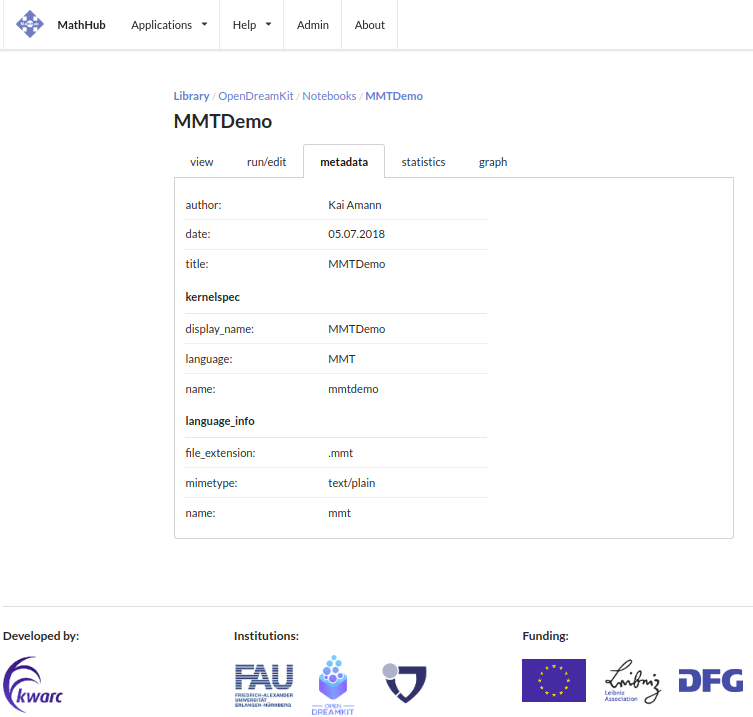
\includegraphics[width=13cm]{NB-Mathhub}}
  \caption{A Jupyter Notebook in MathHub.info (Metadata)}\label{fig:mathhub-NB}
\end{figure}

A displayed Jupyter Notebook additionally has a special button that lets the reader open the notebook in the associated Jupyter server.\ednote{MK@KA: does this use the running MMT process on MathHub.info? That would give the kernel access to the whole MathHub universe --> describe that as a feature.}
\ednote{@Kai, @Tom: check this, do the implementation}

\ednote{KA: write some demo notebooks stored in gl.mathhub.info, including the one corresponding to the example in the previous section}

\ednote{KA: show a screenshot of the example notebook from the previous section in jupyter.mathhub.info}


%%% Local Variables:
%%% mode: latex
%%% mode: visual-line
%%% fill-column: 5000
%%% TeX-master: "report"
%%% End:

%  LocalWords:  Jupyter ednote
